\documentclass{beamer}
\usepackage[orientation=portrait, size=a0, scale = 1.25]{beamerposter}
\usepackage{graphicx}  % Required for including images
\usepackage{booktabs} % Top and bottom rules for tables
\usepackage{subcaption}
\usepackage{tikz}
\usepackage{epstopdf}
\setlength{\leftmargini}{5cm}

\usetheme{confposter} 
        
\newlength{\sepwid}
\newlength{\onecolwid} 
\newlength{\twocolwid}
\newlength{\threecolwid}
\setlength{\sepwid}{0.024\paperwidth} % Separation width (white space) between columns
\setlength{\onecolwid}{0.45\paperwidth} % Width of one column
\setlength{\twocolwid}{0.464\paperwidth} % Width of two columns
\setlength{\threecolwid}{0.708\paperwidth} % Width of three columns
\setlength{\topmargin}{-0.5in} % Reduce the top margin size
 
\title{Data-Driven Lightweight Encoding Selection}
\author{Hao Jiang, Aaron J. Elmore} % Author(s)
\institute{Department of Computer Science\\ The University of Chicago} %
\date{}
% Institution(s)    
\addtobeamertemplate{headline}{} 
{
\begin{tikzpicture}[remember picture,overlay] 
\node [shift={(6.5cm,-3.5cm)}] at (current page.north west)
{
\includegraphics[scale=0.4]{./img/logo_rgb_maroon}};
\node [shift={(7cm,-9cm)}] at (current page.north west)
{
\includegraphics[scale=0.3]{./img/ceres-logo}};
\end{tikzpicture}  
}
\begin{document}  
 


\begin{frame}[t] % The whole poster is enclosed in one beamer frame
 
\usebeamerfont{block body}
\begin{beamercolorbox}[colsep*=2ex,vmode]{block body}
\leftskip4cm
\rightskip4cm

This project explores an automated method to select efficient lightweight
encoding schemes for column-based databases. Existing
methods either rely on database administrators' experience or use simple rules
to make selection. In practice, neither of these methods achieve optimal
performance. We propose a method to solve the problem in a systematic
data-driven way.
 

\end{beamercolorbox}

\begin{columns}[t] 
% The whole poster consists of three major columns, the second of which is
% split into two columns twice - the [t] option aligns each column's content to the top
\begin{column}{\sepwid}\end{column} % Empty spacer column

\begin{column}{\onecolwid} % The first column
          
\begin{block}{Lightweight Encoding}
Popular Lightweight encoding schemes includes Run-Length Encoding, Dictionary
Encoding, Bit-Packing and Delta Encoding. Comparing to popular compression
techniques like gzip and snappy, lightweight encoding schemes have many
advantanges such as Encoding Speed, Local Computation and Support to In-Site
Query Execution.

Best encoding scheme given a data attributes is determined by many
factors including data type and data nature, and there is no simple rule on
how to choose it. The system we propose includes the following features:
\begin{enumerate}\setlength{\itemindent}{1.5em}
  \item Dataset Analysis
  \item Pattern Mining
  \item Data-Driven Encoding Prediction
\end{enumerate}
\end{block}


\begin{block}{Dataset Analysis}
We have created an automated framework to collect datasets, extract columns from
them, organize, and persist the records for further analysis. Using this
framework, we have collected over 7000 columns from approximately 1200 datasets
with a total size of 500G data. These datasets are all from real-world data
sources and cover a rich collection of data types (integer, date, address,
etc.), with diverse data distributions. We use Apache Parquet's built-in
encoders to encode these data columns with different encoding schemes, looking
for the one performing best for each column.

\begin{figure}
\begin{subfigure}{0.5\textwidth}
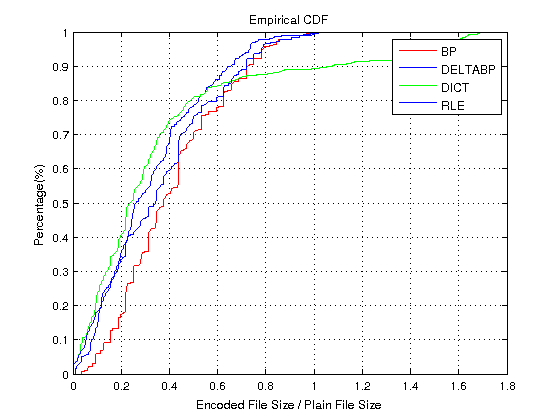
\includegraphics[scale=1.2]{img/integer_cdf}
\caption{Encoding Compression Ratio for Integer Columns}
\end{subfigure}~
\begin{subfigure}{0.5\textwidth}
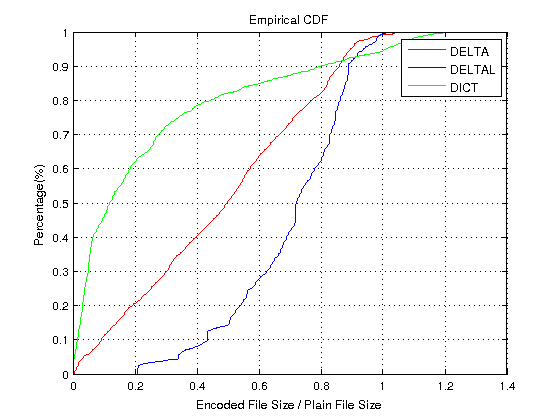
\includegraphics[scale=1.2]{img/string_cdf}
\caption{Encoding Compression Ratio for String Columns}
\end{subfigure}
\end{figure}

\begin{figure}
\begin{subfigure}{0.5\textwidth}
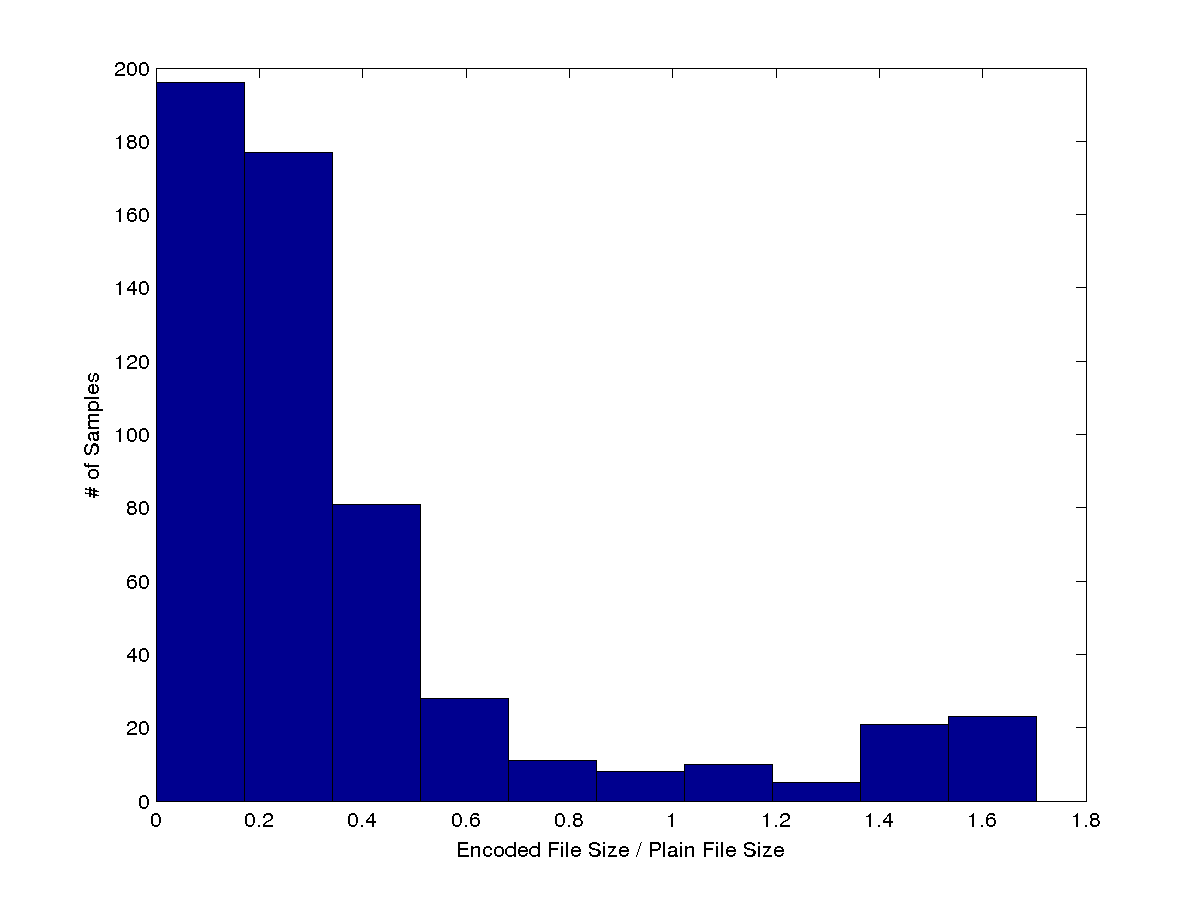
\includegraphics[scale=1]{img/integer_dict_hist}
\caption{Dictionary Encoding for Integer Columns}
\end{subfigure}~
\begin{subfigure}{0.5\textwidth}
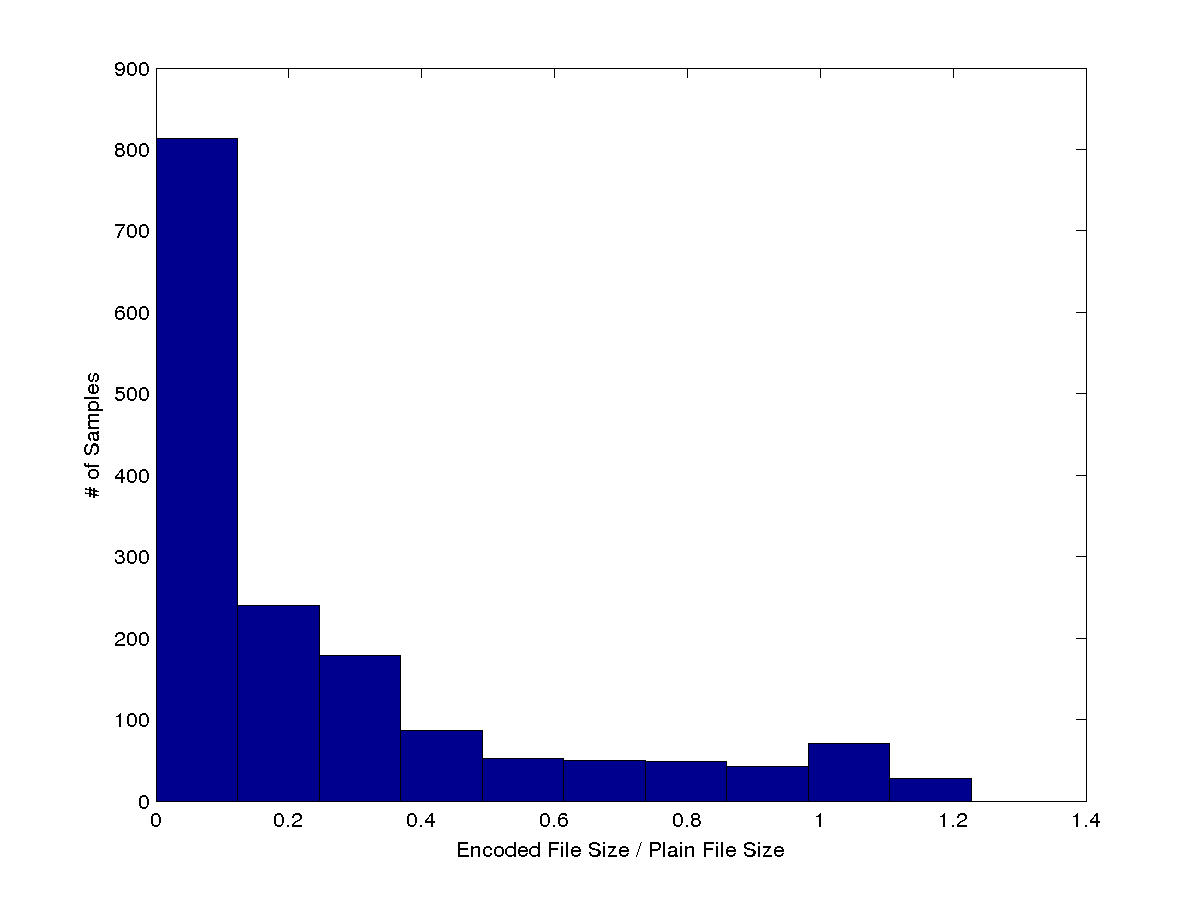
\includegraphics[scale=1]{img/string_dict_hist}
\caption{Dictionary Encoding for String Columns}
\end{subfigure}
\end{figure}

\end{block}

\end{column}

\begin{column}{\sepwid}\end{column} % Empty spacer column

\begin{column}{\onecolwid} % The first column

\begin{block}{Pattern Mining}
Data type is crucial to encoding selection. A proper data type determination
can greatly reduce space requirement for encoded data. For example, storing a
date field in string format requires at least 8 bytes, while storing it in
integer format takes no more than 4 bytes. If we further observe the effective
data range, this can be further reduced to 23 bits. However, most real-world
datasets are semi-structured, in which only part of the data contains valid
common structures. Pattern Mining targets at automatically identify and extract
these structures, allowing more efficient encoding to be applied on them. In
this project, we have developed two methods for Pattern Mining, **Common
Sequence** and **Frequent Similar Words**.


\end{block}

\begin{block}{Data Driven Encoding Prediction}

\end{block}

\end{column}


\begin{column}{\sepwid}\end{column} % Empty spacer column

\end{columns}

\end{frame}
\end{document}